
\documentclass{article}
\usepackage[margin=3cm,a4paper]{geometry}
\usepackage{fancyvrb}
\usepackage{color}
\usepackage{colortbl}
\usepackage[utf8]{inputenc}
\usepackage[scaled=.8]{beramono}
\usepackage[T1]{fontenc}
\usepackage{graphicx}
\usepackage{amsmath}			% packages to give lots of maths stuff
\usepackage{amssymb}
\usepackage[parfill]{parskip}
\usepackage{titlesec}
\usepackage[titletoc,toc,title]{appendix}
\usepackage{tikz}
%\usepackage{dsfont}
\usepackage[autostyle]{csquotes} 

\usepackage[hang,small,bf]{caption}
\setlength{\captionmargin}{30pt}

\usepackage{subcaption}
\captionsetup[subfigure]{labelformat=simple}
\renewcommand\thesubfigure{(\alph{subfigure})}

\usepackage{natbib}
\bibpunct{(}{)}{;}{a}{,}{,}

\usepackage{enumitem}
\setenumerate[1]{label=(\arabic*)}

% default font. 
% can be \sfdefault, \sfdefault or \ttdefault
%\renewcommand*{\familydefault}{\sfdefault}

%%%%%%%%%%%%%%%%%%%%% CREATE COMMANDS HERE %%%%%%%%%%%%%%%%%%%%%%


\definecolor{linkblue}{rgb}{0.192,0.494,0.675}
\definecolor{lghtGrey}{gray}{0.9}
\newcolumntype{g}{>{\columncolor{lghtGrey}}c}
\newcolumntype{C}[1]{>{\centering\let\newline\\\arraybackslash\hspace{0pt}}m{#1}}

\newcommand{\webtext}[1]{\textcolor{linkblue}{\texttt{\footnotesize{#1}}}}
\newcommand{\byme}{\vspace{10mm}\begin{flushright}\footnotesize{Ty Stanford\\ \today}\end{flushright}\vspace{10mm}}

%TiKZ outlined box, good for highlighting important text/tables etc
\tikzstyle{custbox} = [draw=black, fill=black!5,  
	very thick, rectangle, rounded corners, inner sep=6pt, inner ysep=6pt]
\def\tikzbox#1{\vskip3pt\begin{tikzpicture}\node[custbox](box){%
\begin{minipage}{0.5\textwidth}#1\end{minipage}};\end{tikzpicture}\vskip3pt}

\newenvironment{datasection}{\footnotesize\ttfamily}{\par}
% \begin{datasection} ... \end{datasection}


%%%%%%%%%%%%%%%%%%%%% STYLE FILE GENERATION (PYGMENTS CODE) %%%%%%%%%%%%%%%%%%%%%%
%run is working dir: 
% THISSTYLE='paraiso-light'; pygmentize -f tex -S $THISSTYLE -a .syntax > style.tex
%\input{fig/style.tex} 



\begin{document}

%\thispagestyle{empty}


\section*{Title}

\tableofcontents

\clearpage


I am citing \cite{author1999}, see file: \texttt{fig/bib.bib}.

\bigskip

This is how you reference a figure: Figure~\ref{fig:one}.

\bigskip

This is how you reference a subfigure: Figure~\ref{fig:sf2}.

\bigskip

This is how you reference a table: Table~\ref{tab:one}.

\bigskip


%%%%%%%%%%%%%%%%%%%%% QUOTES %%%%%%%%%%%%%%%%%%%%%%

Now for a quote:
\begin{displayquote}
\textsl{Some quote.}
\end{displayquote}
-- some person

%%%%%%%%%%%%%%%%%%%%% FIGURE %%%%%%%%%%%%%%%%%%%%%%

\begin{figure}[h!]
 \centering
   
\includegraphics[width=0.2\textwidth]{fig/corr.pdf}
 \caption{Figure. Words.} \label{fig:one}
\end{figure}



%%%%%%%%%%%%%%%%%%%%% SUB-FIGURES %%%%%%%%%%%%%%%%%%%%%%

\begin{figure}[h!] 
\centering
\begin{subfigure}[b]{0.2\textwidth}
\centering
	\raisebox{0.8\height}{
		
\includegraphics[width=1\textwidth]{fig/corr.pdf}
	}
	\caption{Subcap1. } \label{fig:sf1}
\end{subfigure}
\begin{subfigure}[b]{0.79\textwidth}
\centering 
		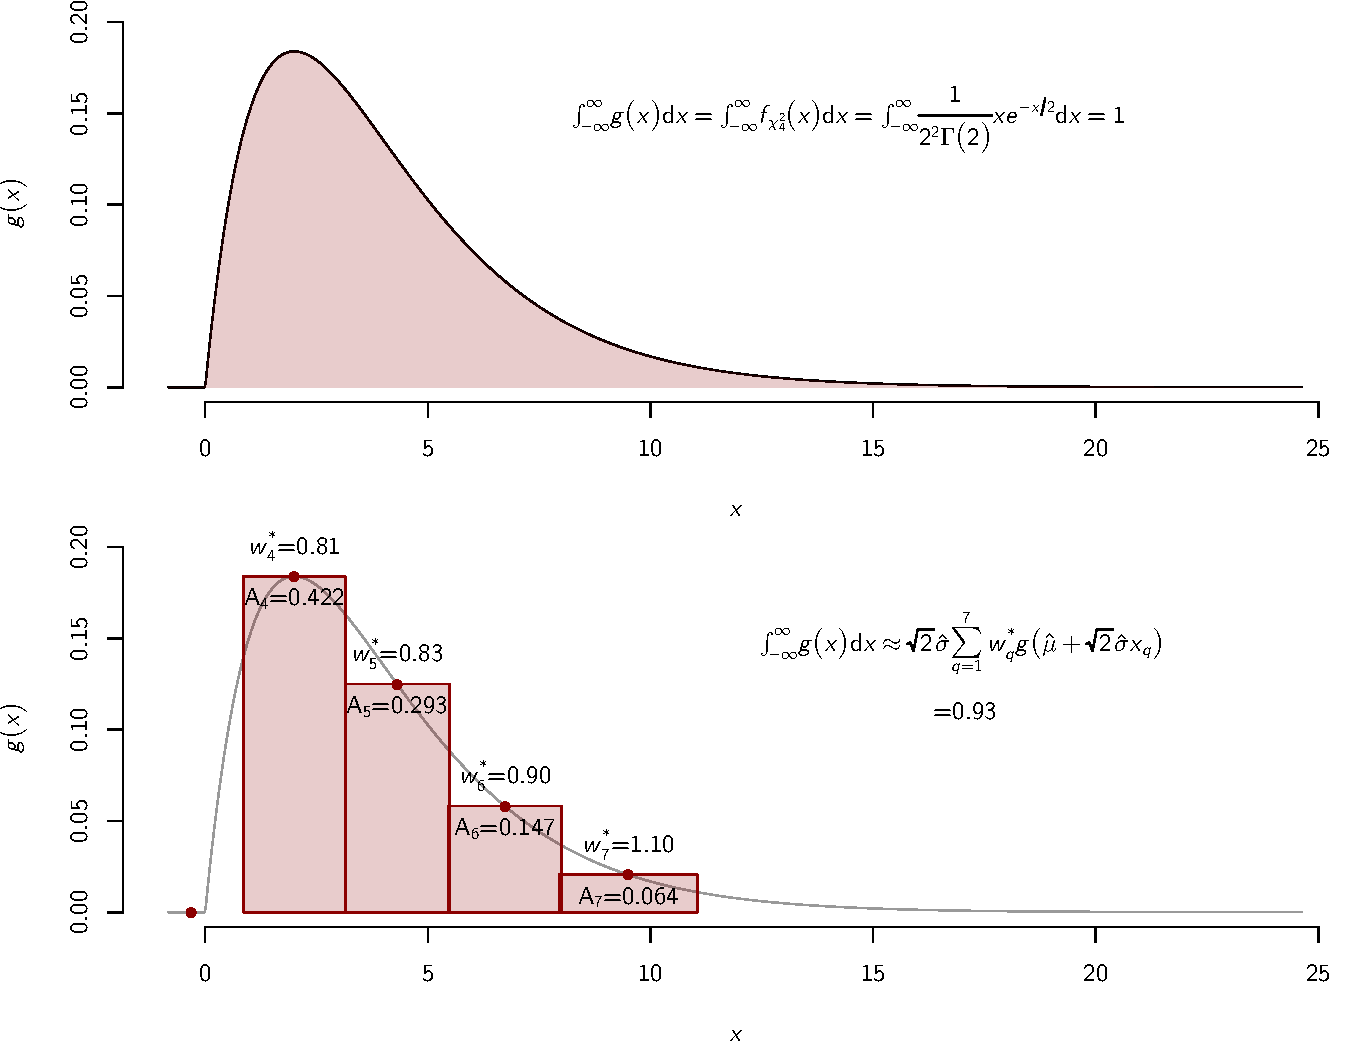
\includegraphics[width=1\textwidth]{fig/g-int-example.pdf}
	\caption{Subcap2. } \label{fig:sf2}
\end{subfigure}
\caption{Bottom caption.} \label{fig:two}
\end{figure}



%%%%%%%%%%%%%%%%%%%%% TABLE %%%%%%%%%%%%%%%%%%%%%%
\begin{table}[ht]
\centering
\caption{Table. Words.} \label{tab:one}
\begin{tabular}{rr}
 \hline
location & p.value \\ 
 \hline
57 & 0.0013 \\ 
  \hline
\end{tabular}
\end{table}


%%%%%%%%%%%%%%%%%%%%% TABLE WITH SHADING %%%%%%%%%%%%%%%%%%%%%%
\begin{table}[ht]
\centering
\caption{Table. Words.}
\begin{tabular}{rC{5cm}}
 \hline
location & p.value \\ 
 \hline
\rowcolor{lghtGrey} 57 & 0.0013 \newline 0.16558 \\ 
  \hline
\end{tabular}
\end{table}

\clearpage

%%%%%%%%%%%%%%%%%%%%% APPENDIX %%%%%%%%%%%%%%%%%%%%%%
\titleformat{\section}{\large\bfseries}{\appendixname~\thesection .}{0.5em}{}
\begin{appendices}

\section{Some Appendix}

$$
\sum_{i=1}^n i^2 
= 
\frac{
n (n+1) (2n+1)
}{
6
}
$$

\end{appendices}


%%%%%%%%%%%%%%%%%%%%% REFENCES %%%%%%%%%%%%%%%%%%%%%%
\bibliographystyle{plainnat}
\bibliography{fig/bib} 

\end{document}












